\documentclass [a4paper,12pt]{article}

\usepackage{pgfplots}
\usepackage{pgfplotstable}
\usepackage{graphicx}
\usepackage{tikz} 
\usepackage[left=2cm,right=2cm, top=2cm,bottom=2cm,bindingoffset=0cm]{geometry}
\usepackage [utf8x] {inputenc}
\usepackage [T2A] {fontenc}
\usepackage {ascii}
\usepackage [english, russian] {babel}
\usepackage {color}
\usepackage {amsmath, amsfonts, amssymb, amsthm, mathtools}
\usepackage {float}
\usepackage{hyperref}
\begin{document}

\begin{titlepage}
\begin{center}
	\large{Московский физико-технический институт}\\
	\vspace{100px}
	\LARGE{Лабораторная работа 3.3.4}\\
	\LARGE{Эффект Холла}\\
	\vspace{30px}
	
\includegraphics[scale = 0.3]{fakt_logo.png}\\
\end{center}

\vfill
\begin{flushright}
	\text{Коваленко Николай}\\
	\text{17.11.2021}\\
	\text{г. Долгопрудный}
\end{flushright}
\end{titlepage}

\newpage

\tableofcontents

\section{Общие сведения}
\subsection{Цель работы}
Измерение постоянной Холла и удельной проводимости полупроводника.

\subsection{Оборудование}
Электромагнит с источником питания, батарейка, амперметр, реостат, цифровой вольтметр, милливеберметр, образцы легированного германия.

\begin{figure}[H]
    \noindent\centering{
        \hspace{-0mm}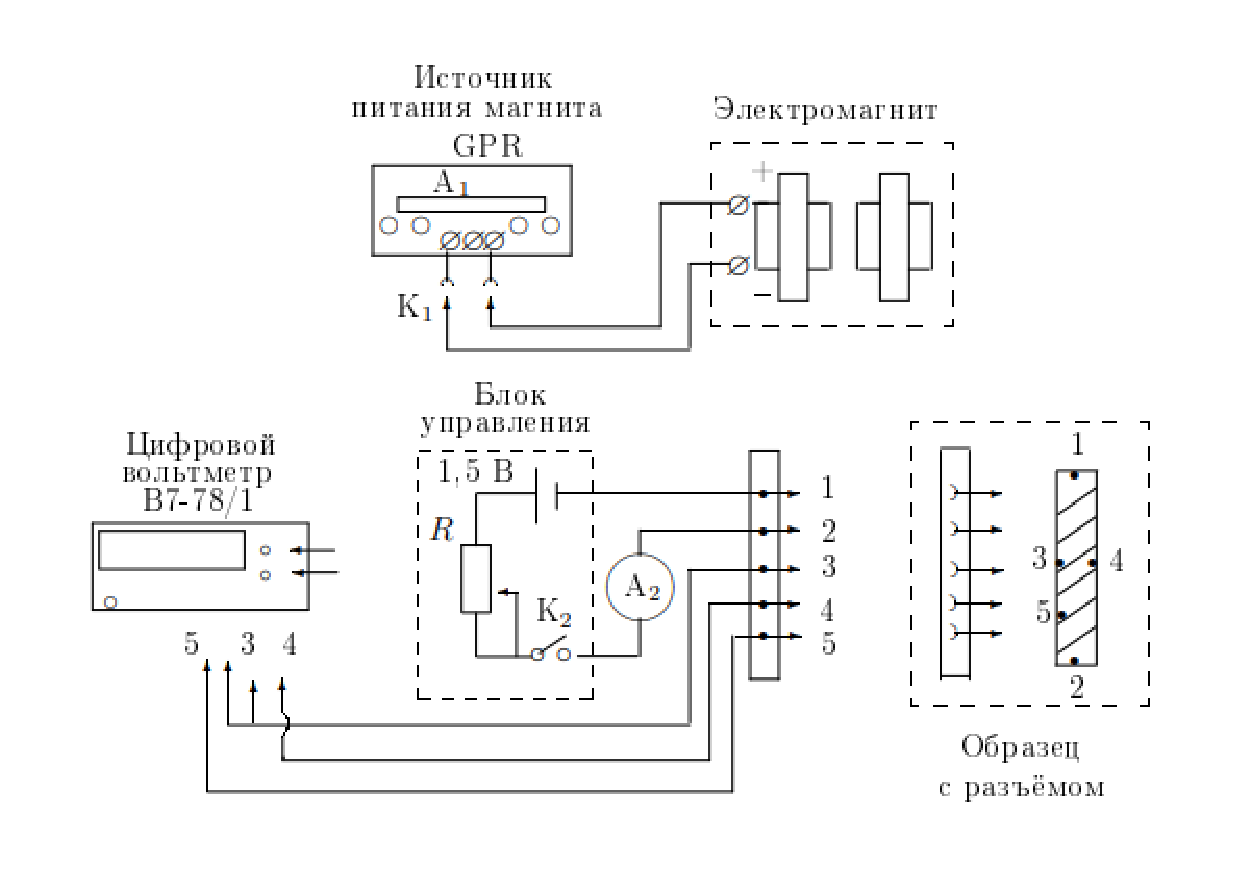
\includegraphics[scale = 0.7]{Station.pdf}
    }
    \caption{Экспериментальная установка.}
    \label{pic1:ref}
\end{figure}

\section{Ход работы}
\subsection{Градуировка электромагнита}

\begin{table}[H]
\caption{\label{tab:canonsummary} Зависимость индукции магнитного поля в зазоре электромагнита B от силы тока $I_m$.}
\begin{center}
\begin{tabular}{|c|c|c|c|c|c|c|c|}
\hline
$\phi$, мВб & 6.5 & 6.3 & 5.8 & 4.8 & 3.7 & 1.9\\
\hline
$I_m$, А & 1.58 & 1.41 & 1.15 & 0.88 & 0.66 & 0.32\\
\hline
B, мТл & 866.67 & 840.00 & 773.33 & 640.00 & 493.33 & 253.33\\
\hline
\end{tabular}
\end{center}
\label{table1:ref}
\end{table}

\begin{center}
\begin{tikzpicture}[baseline]
\begin{axis}[
    title = \text{Зависимость индукции магнитного поля в зазоре электромагнита B от силы тока $I_m$},
    legend pos = north west,
    xlabel = {$I_m$, А},
    ylabel = {B, мТл},
    width = 0.7\textwidth,
    height = 0.45\textwidth,
    %ymin = 6,
    %ymax = 15,
    %xmin = 4,
    %xmax = 22,
]
\addplot[red, domain = 0.2:1.65] {688.124 + 434.572*(ln(x))};
\addplot[blue, domain = 0.2:1.65] {691.7923*x+33.3110};
\addlegendentry{$y = 688.12 + 434.57\cdot ln(x)$};
\addlegendentry{$y = 691.79x + 33.31$};
\addplot[blue, only marks, error bars/.cd, y dir=both, y explicit] 
table[x = X, y = Y, y error = Ey]
{
X   Y   Ey
0.88 639.9999999999999 31.999999999999996
0.66 493.3333333333333 24.666666666666668
0.32 253.33333333333331 12.666666666666666
};
\addplot[
    red,
    only marks,
    error bars/.cd, y dir=both, y explicit,
] 
table[
    x = X,
    y = Y,
    y error = Ey,
]
{
X   Y   Ey
1.58 866.6666666666666 43.333333333333336
1.41 839.9999999999999 42.0
1.15 773.3333333333333 38.666666666666664
};
\end{axis}
\end{tikzpicture}
\end{center}

\subsection{Измерение ЭДС Холла}

\begin{table}[H]
\caption{\label{tab:canonsummary} Рассчет величины ЭДС Холла.}
\begin{center}
\begin{tabular}{|c|c|c|c|c|c|c|c|}
\hline
I = 0.3 мА&&&&&&\\
\hline
$I_m$, А & 0.31 & 0.60 & 0.88 & 1.03 & 1.22 & 1.57 \\
\hline
B, мТл & 247.77 & 448.39 & 642.09 & 745.86 & 877.30 & 1119.42 \\ 
\hline
$\varepsilon_x$, мВ & -0.04 & -0.07 & -0.10 & -0.12 & -0.13 & -0.14 \\ 
\hline
I = 0.4 мА&&&&&&\\
\hline
$I_m$, А & 0.30 & 0.60 & 0.81 & 1.06 & 1.27 & 1.57 \\
\hline
B, мТл & 240.85 & 448.39 & 593.66 & 766.61 & 911.89 & 1119.42 \\
\hline
$\varepsilon_x$, мВ & -0.05 & -0.09 & -0.12 & -0.15 & -0.17 & -0.18 \\ 
\hline
I = 0.5 мА&&&&&&\\
\hline
$I_m$, А & 0.33 & 0.60 & 0.74 & 0.93 & 1.31 & 1.57 \\ 
\hline
B, мТл & 261.60 & 448.39 & 545.24 & 676.68 & 939.56 & 1119.42\\ 
\hline
$\varepsilon_x$, мВ & -0.06 & -0.12 & -0.14 & -0.17 & -0.21 & -0.23 \\
\hline
I = 0.6 мА&&&&&&\\
\hline
$I_m$, А & 0.22 & 0.40 & 0.61 & 0.95 & 1.36 & 1.56 \\ 
\hline
B, мТл & 185.51 & 310.03 & 455.30 & 690.51 & 974.15 & 1112.51 \\ 
\hline
$\varepsilon_x$, мВ & -0.05 & -0.09 & -0.14 & -0.21 & -0.26 & -0.28 \\ 
\hline
I = 0.7 мА&&&&&&\\
\hline
$I_m$, А & 0.27 & 0.61 & 0.90 & 1.20 & 1.37 & 1.57 \\
\hline
B, мТл & 220.09 & 455.30 & 655.92 & 863.46 & 981.07 & 1119.42 \\ 
\hline
$\varepsilon_x$, мВ & -0.07 & -0.16 & -0.23 & -0.28 & -0.30 & -0.32 \\
\hline
I = 0.8 мА&&&&&&\\
\hline
$I_m$, А & 0.30 & 0.60 & 0.72 & 1.05 & 1.25 & 1.57 \\
\hline
B, мТл & 240.85 & 448.39 & 531.40 & 759.69 & 898.05 & 1119.42 \\ 
\hline
$\varepsilon_x$, мВ & -0.09 & -0.19 & -0.22 & -0.30 & -0.33 & -0.37 \\
\hline
I = 0.9 мА&&&&&&\\
\hline
$I_m$, А & 0.33 & 0.60 & 0.81 & 1.07 & 1.37 & 1.56\\
\hline
B, мТл & 261.60 & 448.39 & 593.66 & 773.53 & 981.07 & 1112.51 \\ 
\hline
$\varepsilon_x$, мВ & -0.18 & -0.27 & -0.34 & -0.41 & -0.46 & -0.48 \\ 
\hline
I = 1 мА&&&&&&\\
\hline
$I_m$, А & 0.33 & 0.60 & 0.76 & 1.06 & 1.32 & 1.57 \\ 
\hline
B, мТл & 261.60 & 448.39 & 559.07 & 766.61 & 946.48 & 1119.42\\ 
\hline
$\varepsilon_x$, мВ & -0.19 & -0.30 & -0.36 & -0.45 & -0.50 & -0.53 \\ 
\hline
\end{tabular}
\end{center}
\label{table1:ref}
\end{table}

\begin{center}
\begin{tikzpicture}[baseline]
\begin{axis}[
    title = \text{Зависимость величины ЭДС Холла $\varepsilon_x$ от индукции поля в зазоре электромагнита.},
    legend pos = north west,
    xlabel = {B, мТл},
    ylabel = {$\varepsilon_x$, мВ},
    width = 0.8\textwidth,
    height = 1\textwidth,
    %ymin = 6,
    %ymax = 15,
    %xmin = 4,
    %xmax = 22,
]
\addplot[red, domain = 100:900] {0.00739363 + 0.000147073*x^1};
\addplot[orange, domain = 100:900] {-0.0054405 + 0.000216168*x^1};
\addplot[yellow, domain = 100:900] {-0.00792101 + 0.000275459*x^1};
\addplot[lime, domain = 100:900] {-0.00896124 + 0.000325906*x^1};
\addplot[green, domain = 100:900] {-0.0100594 + 0.000367437*x^1};
\addplot[cyan, domain = 100:900] {-0.0142157 + 0.000442922*x^1};
\addplot[blue, domain = 100:900] {0.0540736 + 0.000483088*x^1};
\addplot[purple, domain = 100:900] {0.0492212 + 0.000556582*x^1};
\addlegendentry{I = 0.3 A, y = (73.9  + 1.47x)$\cdot 10^{-4}$};
\addlegendentry{I = 0.4 A, y = (-54.4 + 2.16x)$\cdot 10^{-4}$};
\addlegendentry{I = 0.5 A, y = (-79.2 + 2.75x)$\cdot 10^{-4}$};
\addlegendentry{I = 0.6 A, y = (-89.6 + 3.26x)$\cdot 10^{-4}$};
\addlegendentry{I = 0.7 A, y = (-100  + 3.67x)$\cdot 10^{-4}$};
\addlegendentry{I = 0.8 A, y = (-142  + 4.43x)$\cdot 10^{-4}$};
\addlegendentry{I = 0.9 A, y = (540.7 + 4.83x)$\cdot 10^{-4}$};
\addlegendentry{I = 1.0 A, y = (492.2 + 5.57x)$\cdot 10^{-4}$};
\addplot[red, only marks, error bars/.cd, y dir=both, y explicit] 
table[x = X, y = Y, y error = Ey]
{
X   Y   Ey
247.76661299999998 0.044 0.0008799999999999999
448.3863799999999 0.073 0.00146
642.088224 0.102 0.0020399999999999997
745.857069 0.117 0.00234
};
\addplot[orange, only marks, error bars/.cd, y dir=both, y explicit] 
table[x = X, y = Y, y error = Ey]
{
X   Y   Ey
240.84868999999998 0.046 0.00092
448.3863799999999 0.093 0.00186
593.662763 0.122 0.00244
766.6108380000001 0.153 0.0030600000000000002
};
\addplot[yellow, only marks, error bars/.cd, y dir=both, y explicit] 
table[x = X, y = Y, y error = Ey]
{
X   Y   Ey
261.602459 0.064 0.00128
448.3863799999999 0.11599999999999999 0.00232
545.237302 0.142 0.0028399999999999996
676.6778390000001 0.173 0.00346
};
\addplot[lime, only marks, error bars/.cd, y dir=both, y explicit] 
table[x = X, y = Y, y error = Ey]
{
X   Y   Ey
185.505306 0.051000000000000004 0.00102
310.02792 0.09300000000000001 0.0018600000000000003
455.30430299999995 0.139 0.0027800000000000004
690.513685 0.21000000000000002 0.004200000000000001
};
\addplot[green, only marks, error bars/.cd, y dir=both, y explicit] 
table[x = X, y = Y, y error = Ey]
{
X   Y   Ey
220.094921 0.06999999999999999 0.0014
455.30430299999995 0.159 0.00318
655.92407 0.23 0.0046
};
\addplot[cyan, only marks, error bars/.cd, y dir=both, y explicit] 
table[x = X, y = Y, y error = Ey]
{
X   Y   Ey
240.84868999999998 0.092 0.00184
448.3863799999999 0.186 0.00372
531.4014559999999 0.22 0.0044
};
\addplot[blue, only marks, error bars/.cd, y dir=both, y explicit] 
table[x = X, y = Y, y error = Ey]
{
X   Y   Ey
261.602459 0.179 0.00358
448.3863799999999 0.274 0.0054800000000000005
593.662763 0.33899999999999997 0.00678
};
\addplot[purple, only marks, error bars/.cd, y dir=both, y explicit] 
table[x = X, y = Y, y error = Ey]
{
X   Y   Ey
261.602459 0.194 0.00388
448.3863799999999 0.30100000000000005 0.006020000000000001
559.0731480000001 0.359 0.00718
};
\end{axis}
\end{tikzpicture}
\end{center}

\begin{center}
\begin{tikzpicture}[baseline]
\begin{axis}[
    title = \text{Зависимость коэффициента k = $\Delta \varepsilon_x / \Delta B$ от силы тока I},
    legend pos = north west,
    xlabel = {$I$, А},
    ylabel = {k, B/Тл},
    width = 0.7\textwidth,
    height = 0.45\textwidth,
    %ymin = 6,
    %ymax = 15,
    %xmin = 4,
    %xmax = 22,
]
\addplot[red, domain = 0.2:1.1] {-1.03205e-005 + 0.000554833*x^1};
\addlegendentry{$y = 5.548\cdot 10^{-4}x$};
\addplot[
    red,
    only marks,
    error bars/.cd, y dir=both, y explicit,
] 
table[
    x = X,
    y = Y,
    y error = Ey,
]
{
X   Y   Ey
0.3 0.000147073 0.000005148
0.4 0.000216168 0.000007566
0.5 0.000275459 0.000009641
0.6 0.000325906 0.000011407
0.7 0.000367437 0.000012860
0.8 0.000442922 0.000015502
0.9 0.000483088 0.000016908
1 0.000556582 0.000019480
};
\end{axis}
\end{tikzpicture}
\end{center}

$$\varepsilon_x = -R_x \frac{I B}{a} \Rightarrow k = -R_x \frac{I}{a} \Rightarrow R_x = - a\frac{k}{I}$$

Значит, $R_x = 0.83 \text{ см}^3\text{/Кл}$

$$\sigma = \frac{I L_{35}}{U_{35} a l}$$

Значит, удельная проводимость $\sigma = 701.11 $Ом/м.

\section{Вывод}
Измерена постоянная Холла $R_x = 0.83 \text{см/Кл}$ и удельная проводимость $\sigma = 701.11 $Ом/м проводника.

\end{document}